\section{Relays: One Circuit Controling Another Circuit}
\label{lab_relays}

%\makelabheader %(Space for student name, etc., defined in master.tex)

\bigskip

\begin{enumerate}[wide]

\item Find the relay in your kit.  (It's a little blue boxy thing, about 1 $\times$ 1 $\times$ 2 cm, with 8 leads.)  
The switch connections are either ``normally open,'' ``normally closed,'' or ``common.''
To actuate the switch, you need to put 5~V across the coil leads, which are pins 1 and 16.
Figure out how the rest of the relay is wired up, by examining the mouse-sized writing on its underside and measuring it with your DMM.
Draw a circuit diagram in your notebook similar to the one on the left below, including pin numbers for all eight leads.    
\begin{center}
\raisebox{0.5in}{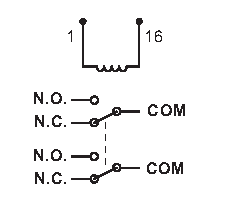
\includegraphics{relays/relay_diagram.eps}}
\hspace{0.6in}
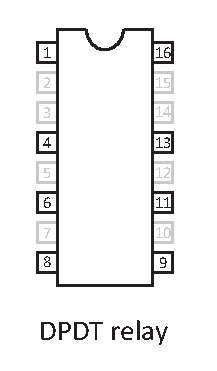
\includegraphics[scale=0.8]{relays/relay_pinout.eps}
\end{center}

\item The switches inside your little relays can safely handle currents of about 1 Amp.  Slightly larger relays, perhaps one cubic inch in volume, can handle currents of 10 or 20 Amps.  By contrast, how large is the current in the coil of your relay?  (Measure it!  It should be a few tens of mA.)

\item Use your 5~V power supply to actuate the relay, opening and closing a circuit that connects your function generator to your speaker.  Draw a good looking diagram of this circuit.

\item Change your circuit so that the relay opens and closes a circuit that connects a 15~VDC power supply to a 10~k$\Omega$ load resistor.  Use your oscilloscope to monitor both the voltage across the relay coil and the voltage across the 10~k$\Omega$ resistor.  Once you apply 5~VDC to the relay coil, how long does it take for the N.O. switch to close?  How long does it take for the N.C. switch to open?  (You should measure a few milliseconds for both.)


\end{enumerate}

\textbf{Possible Exam Questions:}

\begin{itemize}

\item A digital ``AND'' gate is supposed to have a response time of 10 nanoseconds to any change in input.  Describe how you would use an oscilloscope to test this response time.  (How would you trigger, what coupling would you use, etc.) 

\end{itemize}







